\section{Results}
\label{sec:results}
Our meta-model outperforms standard uncertainty estimators in predictive accuracy and cost-aware decision-making across datasets and LLM families. Although we implemented CoT variants, all reported results use direct-answer prompting, as CoT increased confidence without improving calibration.
\subsection{Main Performance Benchmarks: Predictive Accuracy (RQ1)}
\label{subsec:predictive_performance}
Tables~\ref{tab:main_results_public_no_cot} and~\ref{tab:main_results_holdout_no_cot} report F1, AUC-ROC, and Macro-F1 for error prediction across nine LLMs overall, evaluated on two datasets: OpenAI Moderation Dataset~\cite{markov2023holisticapproachundesiredcontent} and a Multimodal Moderation Dataset~\cite{levi+al:25}. The meta-model consistently exceeds MSP, Top-2 Margin, and Entropy baselines.
%main_results_public_set_wo_cot

\begin{table*}[t]
\centering
\caption{Baseline vs.\ meta-model predictive performance on the OpenAI Moderation Dataset. Metrics are reported as percentages. Bold values indicate the best result per metric for each LLM (row-wise).}
\label{tab:main_results_public_no_cot}
\resizebox{\linewidth}{!}{
\begin{tabular}{lcccccccccccc}
\toprule
 & \multicolumn{3}{c}{MSP} & \multicolumn{3}{c}{Top-2 Margin} & \multicolumn{3}{c}{Entropy} & \multicolumn{3}{c}{Meta-Model (Ours)} \\
\cmidrule(lr){2-4} \cmidrule(lr){5-7} \cmidrule(lr){8-10} \cmidrule(lr){11-13}
LLM & F1 & AUC-ROC & Macro-F1 & F1 & AUC-ROC & Macro-F1 & F1 & AUC-ROC & Macro-F1 & F1 & AUC-ROC & Macro-F1 \\
\midrule
gpt-4o-mini         & 81.27\% & 83.55\% & 64.96\% & 81.27\% & 83.55\% & 64.96\% & 80.55\% & 83.43\% & 64.20\% & \textbf{94.14\%} & \textbf{93.46\%} & \textbf{82.31\%} \\
gpt-4o              & 84.35\% & 90.34\% & 71.14\% & 84.41\% & 90.33\% & 70.96\% & 84.35\% & \textbf{90.48\%} & 71.14\% & \textbf{91.35\%} & 90.64\% & \textbf{76.81\%} \\
gpt-4.1-mini        & 88.79\% & 91.10\% & 75.28\% & 88.21\% & 91.04\% & 74.56\% & 88.71\% & 91.07\% & 75.16\% & \textbf{91.93\%} & \textbf{91.73\%} & \textbf{79.94\%} \\
gemini-2.5-flash-lite & 81.04\% & 81.69\% & 65.67\% & 82.70\% & 81.41\% & 66.51\% & 80.95\% & 82.22\% & 65.58\% & \textbf{89.11\%} & \textbf{87.58\%} & \textbf{74.00\%} \\
gemini-2.0-flash-lite & 88.73\% & 85.57\% & 74.52\% & 88.48\% & 85.66\% & 74.26\% & 88.73\% & 85.52\% & 74.52\% & \textbf{93.55\%} & \textbf{89.76\%} & \textbf{81.39\%} \\
gemini-2.0-flash-001  & 85.29\% & 82.76\% & 70.39\% & 85.29\% & 82.76\% & 70.39\% & 85.29\% & 82.76\% & 70.39\% & \textbf{89.38\%} & \textbf{86.34\%} & \textbf{75.36\%} \\
QWEN3-14B  & 90.93\% & 89.94\% & 64.25\% & 90.88\% & 89.90\% & 63.54\% & \textbf{91.07}\% & 89.99\% & 66.52\% & 90.54\% & \textbf{92.07}\% & \textbf{77.20}\% \\

\end{tabular}}
\end{table*}
%main_results_holdout_set_no_cot
\begin{table*}[t]
\centering
\caption{Baseline vs.\ meta-model predictive performance on the Multimodal Moderation Dataset. Metrics are reported as percentages. Bold values indicate the best result per metric for each LLM (row-wise).}
\label{tab:main_results_holdout_no_cot}
\resizebox{\linewidth}{!}{
\begin{tabular}{lcccccccccccc}
\toprule
 & \multicolumn{3}{c}{MSP} & \multicolumn{3}{c}{Top-2 Margin} & \multicolumn{3}{c}{Entropy} & \multicolumn{3}{c}{Meta-Model (Ours)} \\
\cmidrule(lr){2-4} \cmidrule(lr){5-7} \cmidrule(lr){8-10} \cmidrule(lr){11-13}
LLM & F1 & AUC-ROC & Macro-F1 & F1 & AUC-ROC & Macro-F1 & F1 & AUC-ROC & Macro-F1 & F1 & AUC-ROC & Macro-F1 \\
\midrule
gpt-4o-mini         & 85.71\% & 83.87\% & 71.20\% & 85.71\% & 83.95\% & 71.20\% & 85.12\% & 83.69\% & 70.47\% & \textbf{87.34\%} & \textbf{88.71\%} & \textbf{74.07\%} \\
gpt-4o              & 88.05\% & 84.97\% & 67.39\% & 87.58\% & 84.72\% & 66.73\% & 88.00\% & \textbf{84.98\%} & 67.85\% & \textbf{91.42\%} & 84.43\% & \textbf{69.80\%} \\
gpt-4.1-mini        & 88.84\% & \textbf{84.93\%} & \textbf{72.39\%} & 88.84\% & 84.82\% & 72.39\% & 88.84\% & 84.93\% & 72.39\% & \textbf{90.98\%} & 84.18\% & 69.02\% \\
gemini-2.5-flash-lite & 84.53\% & 75.18\% & 63.87\% & 85.28\% & \textbf{75.20\%} & \textbf{64.77\%} & 83.19\% & 75.21\% & 62.81\% & \textbf{90.56\%} & 68.26\% & 57.59\% \\
gemini-2.0-flash-lite & 69.52\% & 67.34\% & 52.41\% & 69.85\% & 67.29\% & 52.67\% & 69.52\% & 67.37\% & 52.41\% & \textbf{85.47\%} & \textbf{69.37\%} & \textbf{61.09\%} \\
gemini-2.0-flash-001      & \textbf{91.65\%} & 62.38\% & 45.82\% & 91.30\% & 62.52\% & 52.17\% & 91.65\% & 62.32\% & 45.82\% & 90.71\% & \textbf{66.37\%} & \textbf{56.47\%} \\
QWEN3-14B            & \textbf{91.06\%} & 74.04\% & 60.04\% & 91.06\% & 73.92\% & 60.04\% & 90.57\% & \textbf{74.25\%} & 60.44\% & 86.49\% & 73.77\% & \textbf{65.97\%} \\
QWEN3-32B            & \textbf{87.70\%} & 74.70\% & 55.10\% & 87.70\% & 74.52\% & 55.10\% & 87.25\% & \textbf{74.79\%} & 54.60\% & 86.82\% & 74.71\% & \textbf{57.69\%} \\
LLAMA32-11B          & \textbf{86.32\%} & \textbf{70.79\%} & 56.02\% & 86.32\% & 70.49\% & 56.02\% & 86.02\% & 70.74\% & 59.68\% & 79.51\% & 70.67\% & \textbf{62.52\%} \\
\bottomrule
\end{tabular}}
\end{table*}

\myparagraph{Text-Only (OpenAI Moderation Dataset)}
The meta-model improves ranking and class balance across models. Relative to the strongest baseline in each row, for \textbf{gpt-4o-mini}, F1 increases from 81.27\% to 94.14\%, AUC-ROC from 83.55\% to 93.46\%, and Macro-F1 from 64.96\% to 82.31\%. Similar improvements are observed for \textbf{gemini-2.5-flash-lite}, where F1 increases from 82.70\% to 89.11\%, AUC-ROC from 82.22\% to 87.58\%, and Macro-F1 from 66.51\% to 74.00\%, and for \textbf{gemini-2.0-flash-lite}, where F1 increases from 88.73\% to 93.55\%, AUC-ROC from 85.66\% to 89.76\%, and Macro-F1 from 74.52\% to 81.39\%. For the stronger-performing models \textbf{gpt-4.1-mini} and \textbf{gpt-4o}, F1 increases from 88.79\% to 91.93\% and from 84.41\% to 91.35\%, respectively. Entries for \textbf{LLAMA32-11B} and \textbf{QWEN3-32B} are omitted from the OpenAI Moderation Dataset results. The former could not be reliably evaluated due to challenges in parsing its outputs across the dataset’s taxonomy, while the latter required compute resources beyond the scope of our evaluation. These omissions do not affect the aggregate trends reported.

\myparagraph{Multimodal (Multimodal Moderation Dataset)}
On the harder Multimodal Moderation Dataset, effects are more model-dependent. For \textbf{gpt-4o-mini}, F1 increases from 85.71\% to 87.34\%, AUC-ROC from 83.95\% to 88.71\%, and Macro-F1 from 71.20\% to 74.07\%. For \textbf{gpt-4o}, F1 increases from 88.05\% to 91.42\%, while Macro-F1 increases from 67.85\% to 69.80\%. The largest gains are observed for \textbf{gemini-2.0-flash-lite}, where F1 increases from 69.85\% to 85.47\% and Macro-F1 from 52.67\% to 61.09\%. In contrast, some models exhibit trade-offs: for \textbf{gpt-4.1-mini}, Macro-F1 decreases from 72.39\% to 69.02\%, and for \textbf{gemini-2.5-flash-lite}, Macro-F1 decreases from 64.77\% to 57.59\%. In several cases (e.g., \textbf{QWEN3-14B}, \textbf{LLAMA32-11B}), F1 decreases despite gains in Macro-F1, indicating calibration challenges and majority-class bias under distribution shift.

\subsection{Cost-Aware Escalation: Operational Efficiency (RQ2)}
\label{subsec:cost_analysis}
Table~\ref{tab:cost_merged_side_by_side} reports expected costs and escalation rates under the cost-aware policy described in Section~\ref{subsec:policy}. These results address RQ2 by quantifying the economic value of selective escalation in production human--AI workflows.
%cost_results_cross_datasets_wo_cot
\begin{table*}[t]
\centering
\caption{Cost-aware evaluation. Metrics: Always-Trust (A.T.) cost (\$), expected cost (\$), escalations (count), and escalation ratio (\%). Bold values indicate the lowest expected cost among methods for each LLM (row-wise).}
\label{tab:cost_merged_side_by_side}
\begin{tabular}{@{}c @{\ \vrule width 1pt\ } c@{}}  % <-- the separator line
% ---------- Left subtable ----------
\begin{subtable}[t]{0.56\linewidth}
\centering
\caption{OpenAI Moderation Dataset}
\label{tab:cost_results_public}
\setlength{\tabcolsep}{2.05pt}
\renewcommand{\arraystretch}{1.05}
\resizebox{\linewidth}{!}{
\begin{tabular}{lccccccccccccc}
\toprule
LLM & A.T. & \multicolumn{3}{c}{MSP} & \multicolumn{3}{c}{Top-2 Margin} & \multicolumn{3}{c}{Entropy} & \multicolumn{3}{c}{Meta-Model (Ours)} \\
 &  & Cost & Esc & Ratio & Cost & Esc & Ratio & Cost & Esc & Ratio & Cost & Esc & Ratio \\
\cmidrule(lr){3-5}\cmidrule(lr){6-8}\cmidrule(lr){9-11}\cmidrule(lr){12-14}
gpt-4o-mini   & 127 & 138   & 339 & 38\% & 132 & 331 & 37\% & 138   & 339 & 38\% & \textbf{38} & 148 & 16\% \\
gpt-4o        & 127 & 74    & 275 & 31\% & 75  & 271 & 30\% & 74    & 275 & 31\% & \textbf{51} & 151 & 17\% \\
gpt-4.1-mini  & 127 & 69    & 258 & 29\% & 73  & 267 & 30\% & 69    & 259 & 29\% & \textbf{45} & 212 & 24\% \\
gemini-2.5-flash-lite & 127 & 128 & 347 & 38\% & 122 & 315 & 35\% & 128 & 348 & 39\% & \textbf{77} & 227 & 25\% \\
gemini-2.0-flash-lite & 127 & 74  & 248 & 28\% & 75  & 253 & 28\% & 74  & 248 & 28\% & \textbf{41} & 162 & 18\% \\
gemini-2.0-flash-001      & 127 & 97  & 297 & 33\% & 97  & 297 & 33\% & 97  & 297 & 33\% & \textbf{69} & 238 & 26\% \\
QWEN3-14B     & 127 &    103   &   73  &   8\%     &   105     &  70   &    8\%    &   98     &  84   &    9\%    &    \textbf{56}   &  205   &   23\%     \\
QWEN3-32B     & NA   & NA       & NA     & NA        & NA        & NA     & NA        & NA        & NA     & NA        & NA       & NA     & NA        \\
LLAMA32-11B   & NA   & NA       & NA     & NA        & NA        & NA     & NA        & NA        & NA     & NA        & NA       & NA     & NA        \\
\bottomrule
\end{tabular}}
\end{subtable}
&
% ---------- Right subtable ----------
\begin{subtable}[t]{0.44\linewidth}
\centering
\caption{Multimodal Moderation Dataset}
\label{tab:cost_results_holdout}
\setlength{\tabcolsep}{2.05pt}
\renewcommand{\arraystretch}{1.05}
\resizebox{\linewidth}{!}{
\begin{tabular}{ccccccccccccc}
\toprule
A.T. & \multicolumn{3}{c}{MSP} & \multicolumn{3}{c}{Top-2 Margin} & \multicolumn{3}{c}{Entropy} & \multicolumn{3}{c}{Meta-Model (Ours)} \\
 & Cost & Esc & Ratio & Cost & Esc & Ratio & Cost & Esc & Ratio & Cost & Esc & Ratio \\
\cmidrule(lr){2-4}\cmidrule(lr){5-7}\cmidrule(lr){8-10}\cmidrule(lr){11-13}
42 & 39 & 110 & 37\% & 37 & 107 & 36\% & 39 & 110 & 37\% & \textbf{22} & 80 & 27\% \\
42 & 41 & 70  & 23\% & 42 & 73  & 24\% & 40 & 72  & 24\% & \textbf{29} & 38 & 13\% \\
42 & 32 & 85  & 28\% & 32 & 85  & 28\% & 32 & 85  & 28\% & \textbf{30} & 40 & 13\% \\
42 & 53 & 93  & 31\% & 51 & 90  & 30\% & 53 & 92  & 31\% & \textbf{40} & 20 & 7\% \\
\textbf{42} & 80 & 163 & 54\% & 80 & 162 & 54\% & 80 & 163 & 54\% & 45 & 64 & 21\% \\
42 & 35 & 7   & 2\%  & 35 & 7   & 2\%  & 35 & 10  & 3\%  & \textbf{34} & 15 & 5\% \\
42 & \textbf{36} & 17 & 6\% & \textbf{36} & 65 & 22\% & \textbf{36} & 21 & 7\% & \textbf{36} & 65 & 22\% \\
\textbf{42} & 47 & 35 & 12\% & 47 & 46 & 15\% & 49 & 37 & 12\% & 47 & 46 & 15\% \\
42 & 41 & 25 & 8\%  & 39 & 78 & 26\% & \textbf{38} & 33 & 11\% & 39 & 78 & 26\% \\
\bottomrule
\end{tabular}}
\end{subtable}
\\ % end row of the 2-col wrapper
\end{tabular}
\end{table*}
\myparagraph{Significant Cost Reductions on Text-Only Benchmark} On the OpenAI Moderation Dataset, the meta-model achieves substantial cost savings relative to standard baselines for most models. For \textbf{gpt-4o-mini}, expected cost decreases from \$132 (best baseline: Top-2 Margin) to \$38 (71\% reduction), while the number of escalations decreases from 331 to 148. Similarly, for \textbf{gemini-2.5-flash-lite}, expected cost decreases from \$122 to \$77 (36\% reduction) and escalations from 315 to 227. For \textbf{gemini-2.0-flash-lite}, expected cost decreases from \$74 to \$41 (41\% reduction), with escalations decreasing from 248 to 162. These patterns indicate that baseline methods (e.g., MSP, Entropy) tend to over-escalate, triggering unnecessary human reviews that inflate operational costs without proportional gains in error prevention. In contrast, the meta-model’s improved calibration enables more targeted escalation, reducing false alarms while preserving error detection.\footnote{Costs are reported in \$, based on estimated review time and projected business loss per error; exact values are task-dependent and we report relative comparisons.}
\myparagraph{Generalization to Multimodal Workflows} The Multimodal Moderation Dataset exhibits similar trends with notable variation across models. For \textbf{gpt-4o-mini}, expected cost decreases from \$37 (best baseline: Top-2 Margin) to \$22 (41\% reduction), with escalations decreasing from 107 to 80. \textbf{gpt-4o} shows a comparable pattern, with expected cost decreasing from \$42 to \$29 (32\% reduction) and escalations from 73 to 38. Notably, for \textbf{gemini-2.5-flash-lite}, expected cost decreases from \$51 to \$40 (22\% reduction) while the number of escalations decreases from 90 to 20. These results suggest that the meta-model can exploit modality-specific uncertainty signals (e.g., visual ambiguity vs.\ transcript inconsistency) that single-metric baselines fail to capture. However, not all models benefit uniformly: for \textbf{QWEN3-14B} and \textbf{LLAMA32-11B}, expected cost remains comparable to the Top-2 Margin baseline, indicating limited gains from meta-modeling on this dataset.
\subsection{Feature Family Ablations: Decomposing LPP Contributions}
\label{subsec:ablations}
To quantify the individual contributions of each LPP family, we conduct systematic ablation studies where the meta-model is trained with one feature group removed. Figures~\ref{fig:ablation_public_no_cot} and~\ref{fig:ablation_holdout_no_cot} visualize the resulting cost increases relative to the full model across base LLMs.
\myparagraph{Complementary Nature of Feature Families}
Across all settings, removing \emph{any} feature family degrades performance, confirming that the three LPP groups (Post-Hoc Classification Uncertainty, Verbalized Confidence, and Uncertainty Attribution Indicators) capture complementary aspects of model behavior.
In Figures~\ref{fig:ablation_public_no_cot} and~\ref{fig:ablation_holdout_no_cot}, these correspond respectively to \emph{Outcome-Level}, \emph{Verbalized}, and \emph{Inconclusive} feature groups.
On the OpenAI Moderation Dataset (Figure~\ref{fig:ablation_public_no_cot}), removing Post-Hoc Classification Uncertainty features (Entropy, MSP, Top-2 Margin) leads to the largest cost increases for most models, consistent with prior work showing that token-level probabilities are the strongest single uncertainty signal.
Removing verbalized confidence also increases costs by roughly 5--15\%, as indicated by the cost differences in Figures~\ref{fig:ablation_public_no_cot} and~\ref{fig:ablation_holdout_no_cot}, suggesting that self-reported confidence adds complementary signals not fully captured by probabilistic features.

The Uncertainty Attribution Indicators, despite being binary, contribute measurably to cost reduction, with especially visible effects for \textbf{gemini-2.5-flash-lite} and \textbf{gemini-2.0-flash-lite}, where removing them produces clear increases in expected costs. This highlights the value of explicit abstention signals in helping the meta-model avoid false confidence—cases where the base LLM assigns high probability to an incorrect answer due to policy ambiguity or evidence deficits.
\begin{figure}[t]
    \centering
    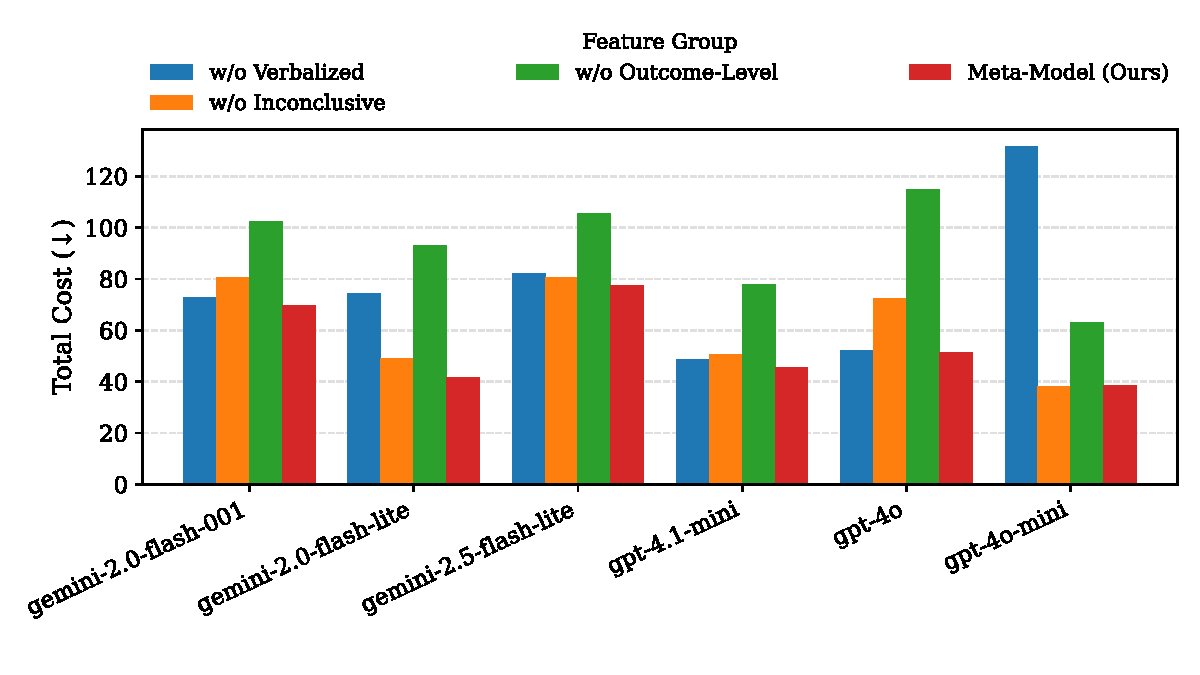
\includegraphics[width=0.9\linewidth]{figures/ablation_public_set_cost_wo_cotablation_holdout_set_cost_wo_cot_pdf.pdf}
    \Description{Bar plot of an ablation study on the OpenAI Moderation Dataset with CoT prompting, where each bar shows the total cost after removing one predictor feature family.}
   \caption{Ablation study on the OpenAI Moderation Dataset. Bars show total cost (\$) when removing one feature family, illustrating each predictor group’s contribution.}
    \label{fig:ablation_public_no_cot}
\end{figure}
\input{figures/ablation_holdout_set_cost_wo_cot}
\subsection{Cross-Dataset Generalization and Robustness}
\label{subsec:generalization}
A key question for meta-learning is whether patterns transfer across distributions. Our two-dataset evaluation shows \textit{model-dependent} robustness: on the OpenAI Moderation Dataset (text-only), the meta-model consistently outperforms post-hoc baselines, while on the Multimodal Moderation Dataset it improves some models (e.g., gpt-4o-mini, gpt-4o, gemini-2.0-flash-lite) but is matched or outperformed by others (e.g., QWEN, LLAMA), reflecting heterogeneity under domain shift.

Absolute performance naturally degrades for some models when moving from the text-only benchmark to the harder multimodal distribution. For example, for gpt-4.1-mini the Macro-F1 score decreases from \textbf{79.94\%} (text-only) to \textbf{69.02\%}, illustrating the additional complexity introduced by visual ambiguity, multilingual code-switching, and culturally contingent moderation judgments. Despite these shifts, the meta-model retains gains for multiple models on the Multimodal Moderation Dataset, while revealing cases where baseline methods remain competitive, underscoring that generalization depends on both the base LLM family and the evaluation distribution.

These patterns reinforce the \emph{cost-aware} view: even when accuracy gains are mixed under distribution shift, LPP-based escalation yields savings by directing review to the most error-prone cases.
\subsection{Limitations and Open Challenges}
\label{subsec:limitations}
Our study demonstrates substantial progress, but several limitations remain. First, the meta-model requires labeled data samples with ground-truth moderation decisions, which introduces annotation costs. Semi-supervised and active learning strategies could reduce this burden. Second, we focus only on \emph{post-response} LPPs extracted after the LLM generates an answer. Incorporating \emph{pre-response} predictors could enable anticipatory escalation and adaptive coordination.
Third, although we evaluate across a range of LLM families, all are transformer-based autoregressive models. Whether LPPs generalize to other architectures (e.g., retrieval-augmented or neuro-symbolic systems) remains an open question. Fourth, our cost model assumes fixed review and error penalties, whereas in practice costs vary by severity, reviewer expertise, and platform-specific risk tolerance. Extending escalation to a dynamic resource-allocation problem is a promising direction.
Finally, while we extracted Chain-of-Thought (CoT) derived features, we do not advocate CoT prompting in this setting: in our experiments, it inflated confidence and harmed calibration~\cite{tian+al:23,zhang2024studycalibrationincontextlearning}.

More broadly, our experiments focus on content moderation, but the LPP framework is applicable to other high-stakes settings such as fraud detection, compliance, or medical triage, where abstention signals and cost-sensitive escalation are equally critical.
\begin{figure}[t]
    \centering
    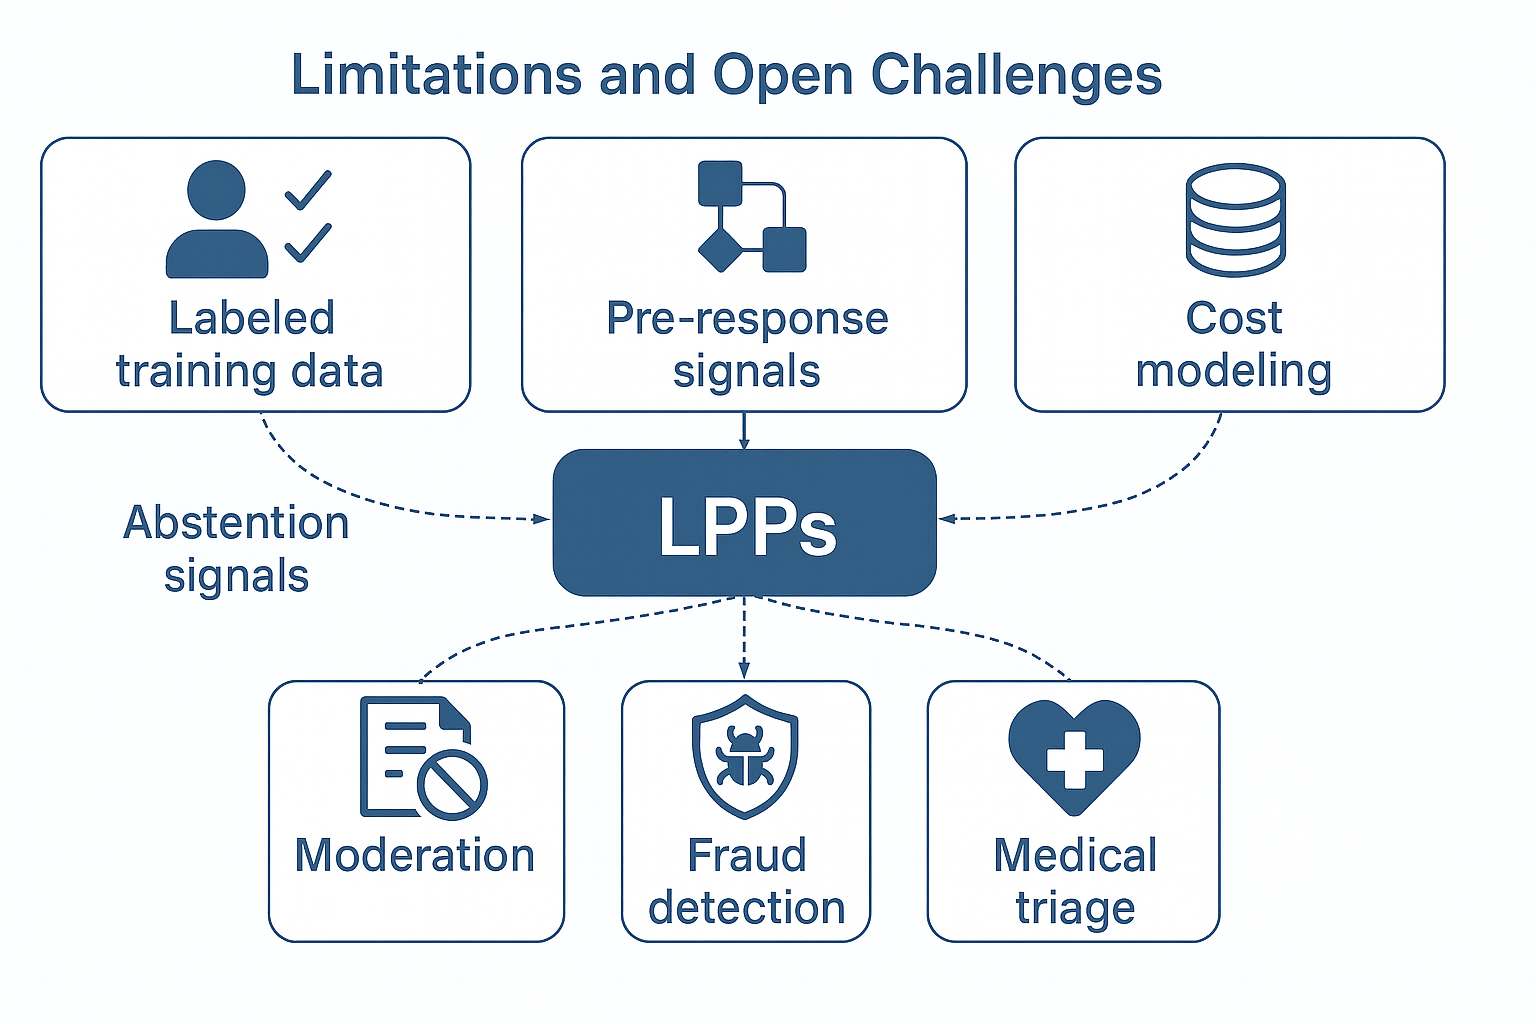
\includegraphics[width=0.9\linewidth]{figures/lpp_cross_domain_router.png}
    \Description{Diagram showing LPPs as the central box connected by arrows to surrounding components. Above, three boxes labeled Labeled training data, Pre-response signals, and Cost modeling feed into LPPs. Below, three boxes labeled Moderation, Fraud detection, and Medical triage receive outputs from LPPs. Dashed arrows indicate abstention signals.}
    \caption{\textbf{LPPs as a cross-domain uncertainty router.} The meta-model routes between automated decisions and human review using uncertainty signals, applicable to moderation, fraud detection, compliance, and medical triage.}
    \label{fig:lpp_router}
    \vspace{-9pt}
\end{figure}
Figure~\ref{fig:lpp_router} illustrates this broader vision: by abstracting uncertainty-aware routing beyond moderation, LPPs can act as a general-purpose coordination mechanism wherever human expertise must be allocated efficiently under uncertainty.
We excluded safety-specialized models like Llama Guard~\cite{Inan2023LlamaGL}, whose taxonomies do not align with our categories (DIMC: Death/Injury/Military Conflict; DAT: Drugs/Alcohol/Tobacco; Kids). Such models may offer stronger abstention signals or calibration, and hybrid setups with domain-specialized safety models are a natural future direction.